% !TEX encoding = UTF-8
%% Vorlage für LEN-Aufgaben
%% Basiert auf der KOMA-Article-Klasse
%% weiter Informationen unter http://www.komascript.de
%%
%% Bei Fragen kannst Du dich auch an die Organisatoren des LaTeX-Einfuerungs-
%% kurses der Fachschaft wenden. Du erreichst uns unter:
%% latex@fachschaft.etec.uni-karlsruhe.de
%% 
%% 2010/11/30 Ferdinand Schwenk
\documentclass[%
  a4paper, %
  12pt, %
   article, %
  titlepage
]{scrartcl}

%% Zeichensatzkodierung 
%% Unter Windows [latin1]
%% Unter Linux [utf8] verwenden.
\usepackage[utf8]{inputenc}
\usepackage[T1]{fontenc}
\usepackage[ngerman]{babel}
 
\usepackage{listings}
\usepackage{color}

%% Zusatz Pakete einbinden
% Zum Einbinden von Quelltexten
\usepackage{listings}
% !TEX encoding = UTF-8
%% Definition der Quelltextformatierung
%% 
%% 2010/11/30 Ferdinand Schwenk
\lstset{%
  language=Matlab,                    % Sprache: Matlab
  numbers=left,                       % Nummerierung: links
  numberstyle=\tiny,                  % Formatierng der Nummerierung
  numbersep=8pt,                      % Abstand der Nummerierung vom Quelltext
  frame=trBL,                         % Rahmen um den Quelltext
  rulecolor=\color{blue},             % Farbe des Rahmens
  rulesepcolor=\color{red},           %
  backgroundcolor=\color[gray]{0.9},  %
  extendedchars=true,                 %
  breaklines=true,                    %
  basicstyle=\scriptsize              %
}
        % Einstellungen für das linstings-Paket laden

% Bilder und Farbe
\usepackage{graphicx}
\usepackage{color}

% Mathematische Formeln
\usepackage{amsmath}

% Tabellen
\usepackage{tabularx}

%% Meta-Informationen
\author{%
\raggedright
  \normalsize %
  \begin{tabularx}{\textwidth}{|l|X|}%
    \hline%
    \textbf{Vorname:}         & Niklas \\ \hline
    \textbf{Nachname:}        & Fauth \\ \hline
    \textbf{Matrikelnummer:}  & 1932872 \\ \hline
    \textbf{RZ-Account:} & utede \\ \hline
    \textbf{Punkte:}          &  \\ \hline % Hier sollst DU wohl nichts eintragen ;-)
  \end{tabularx}%
}
% ------------------------------------------------------------------------------
% Die Informationen in diesem Bereich bitte nicht aendern
% !TEX encoding = UTF-8
% !TEX root = vorlage.tex
%% Erstellt die Titelseite für die LEN-Aufgaben
%% 
%% 2010/11/30 Ferdinand Schwenk
\title{Spice-Aufgabe WS 15/16}
% ------------------------------------------------------------------------------
% Die Informationen in diesem Bereich bitte nicht aendern
\titlehead{%
  \begin{tabularx}{\linewidth}{|>{\centering\arraybackslash}X|>{\centering\arraybackslash}X|}%
    \hline%
    \multicolumn{2}{|c|}{\large Karlsruher Institut f\"ur Technologie} \\
    \multicolumn{2}{|c|}{\large \textbf{Institut f\"ur Biomedizinische Technik}} \\ \hline
    Prof. Dr. rer. nat. O. D\"ossel & M. Sc. M. Kircher \\ & Dipl. Ing. J. Schmid\\
    \scriptsize Kaiserstr. 12 / Geb. 30.33 & \scriptsize Kaiserstr. 12 / Geb. 30.33 \\
    \scriptsize Tel.: 0721 / 608-42650 & \scriptsize Tel.: 0721 / 608-2751 \\
    \hline %
  \end{tabularx}%
}
\subject{Lineare Elektrische Netze}
\date{  }
\publishers{
\raggedright
\normalsize{\underline{Angaben zur Bearbeitung der Aufgaben:}\vspace{0.2cm}\\ 
Die Aufgaben m\"ussen selbstst\"andig und ohne fremde Hilfe bearbeitet werden.\vspace{0.2cm}\\
Der L\"osungsweg muss vollst\"andig angegeben und nachvollziehbar sein! Dokumentieren Sie Ihre \"Uberlegungen, geben Sie erl\"auternde Kommentare!\vspace{0.2cm}\\
Die maximale Punktzahl dieser Aufgabe entspricht 3\% der Gesamtpunktzahl der Endnote im Fach Lineare Elektrische Netze.\\
\vspace{0.8cm}
\textbf{Eidesstattliche Erkl\"arung}\\
\vspace{0.2cm}
Hiermit erkl\"are ich an Eides statt, dass ich die vorliegende
Arbeit  selb\-stst\"andig  und  ohne  unzul\"assige fremde Hilfsmittel angefertigt habe. W\"ortlich oder inhaltlich \"ubernommene Stellen sind als solche kenntlich gemacht und die verwendeten Literaturquellen im Literaturverzeichnis  vollst\"andig angegeben. Die \glqq Regeln zur Sicherung guter wissenschaftlicher Praxis im Karlsruher Institut f\"ur Technologie (KIT)\grqq\, in ihrer g\"ultigen Form wurden beachtet. \\
\vspace{1.5cm}
Karlsruhe, den \rule{10 cm}{0.4pt}
\hspace*{6cm}\footnotesize{{Datum und Unterschrift}}

}}

% ------------------------------------------------------------------------------

% ------------------------------------------------------------------------------

% Hier beginnt das Dokument
\begin{document}
  % Erstellt die Titelseite
  \maketitle

  %Gibt das Inhaltsverzeichnis aus
\begingroup
\let\cleardoublepage\clearpage
\tableofcontents
\endgroup
  %\clearpage
  
  %% Hier kannst du jetzt Deinen Lösungstext schrieben.
  %% Grafiken einbinden (*.pdf oder *.png):
  %%   \includegraphics{Pfad/zu/Deinem/Bild}
  %%   \includegraphics[width=BREITE,height=HOEHE,keepaspectratio]{Pfad/zu/Deinem/Bild}
  %% Quelltext einbinden:
  %%   \lstinputlisting[caption={BESCHRIFTUNG}]{Pfad/zu/deinem/quelltext}





  \section{Einführung}
Nachfolgend die erarbeiteten Lösungen. Zum Teil wurde von einer minimalistischen Lösung abgesehen, um für schöneren Code zu Sorgen oder die Benutzerfreundlichkeit 
zu erhöhen. 

  \section{UDot}
  \subsection{Erklärung}

UDot ist eine eigene Implementierung einer Funktion, um (Spannungs)werte gegenüber der Zeit abzuleiten.


\newpage

 \subsection{Quellcode}




 
\definecolor{codegreen}{rgb}{0,0.6,0}
\definecolor{codepurple}{rgb}{0.58,0,0.82}
\definecolor{backcolour}{rgb}{0.95,0.95,0.92}
 
\lstdefinestyle{mystyle}{  
    commentstyle=\color{codegreen},
    keywordstyle=\color{blue},
    numberstyle=\tiny\color{black},
    stringstyle=\color{codepurple},
    basicstyle=\footnotesize,
    frame=single,	
    breakatwhitespace=false,         
    breaklines=true,                 
    captionpos=b,                    
    keepspaces=true,                 
    numbers=left,                    
    numbersep=5pt,                  
    showspaces=false,                
    showstringspaces=false,
    showtabs=false,                  
    tabsize=2,
    rulecolor=\color{black}
}
 
\lstset{style=mystyle}

Nachfolgend der Quellcode der Funktion UDot.
 
\lstinputlisting[language=Matlab]{UDot.m}

\newpage

Die Funktion erfüllt alle geforderten Bedingungen. Haben die zwei Ausgangsvektoren nicht dieselbe Länge, wird eine entsprechende Warnung ausgegeben.
Um diese Ausnahme abzufangen wird im Fehlerfall jedoch nicht einfach abgebrochen, sondern der kürzere der beiden Vektoren zur Berechnung genutzt.
Die Angabe, welcher Vektor tatsächlich verwendet wurde, ist in der Warnung enthalten.

 \subsection{help-Ausgabe}

Durch Eingabe des Befehls >help UDot< erscheint folgende Hilfe:

\begin{figure}[h]
\fbox{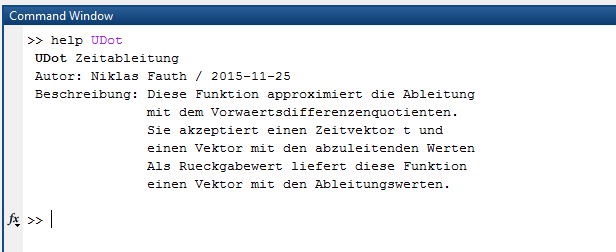
\includegraphics[width=\textwidth]{UDot_help.png}}
\caption{help-Ausgabe}
\label{fig1}
\end{figure}




  \section{UInt}
  \subsection{Erklärung}

UInt ist eine eigene Implementierung einer Funktion, um (Spannungs)werte gegenüber der Zeit zu integrieren.


\newpage

 \subsection{Quellcode}

Nachfolgend der Quellcode der Funktion UInt.
 
\lstinputlisting[language=Matlab]{UInt.m}

\newpage

Die Funktion erfüllt alle geforderten Bedingungen. Haben die zwei Ausgangsvektoren nicht dieselbe Länge, wird eine entsprechende Warnung ausgegeben.
Um diese Ausnahme abzufangen wird im Fehlerfall jedoch nicht einfach abgebrochen, sondern der kürzere der beiden Vektoren zur Berechnung genutzt.
Die Angabe, welcher Vektor tatsächlich verwendet wurde, ist in der Warnung enthalten.

 \subsection{help-Ausgabe}

Durch Eingabe des Befehls >help UInt< erscheint folgende Hilfe:

\begin{figure}[h]
\fbox{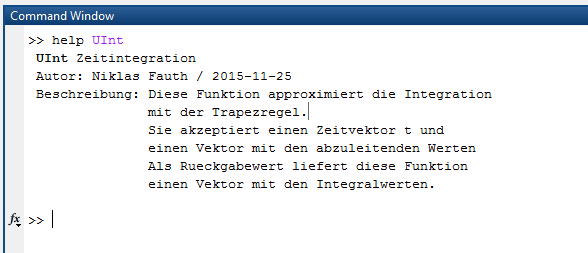
\includegraphics[width=\textwidth]{UInt_help.png}}
\caption{help-Ausgabe}
\label{fig2}
\end{figure}

\newpage

  \section{Anwendung}
  \subsection{Ableiten}

bla bla bla

\begin{figure}[h]
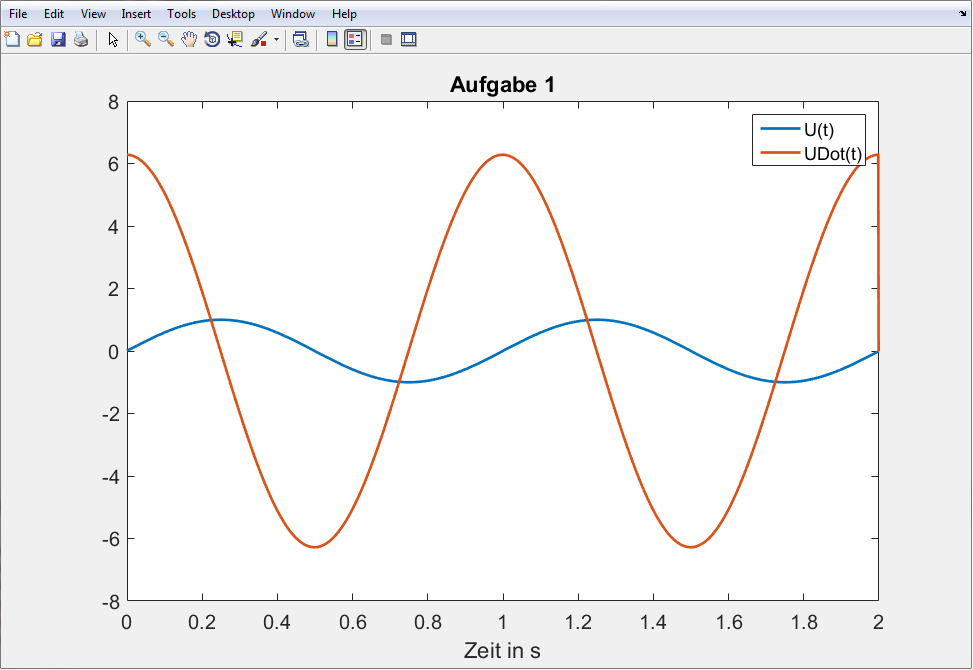
\includegraphics[width=\textwidth]{plot1.png}
\caption{Plot der Ausgangsfunktion und ihrer Ableitungsfunktion}
\label{fig3}
\end{figure}

Dazu wurden folgende Befehle verwendet:

\lstinputlisting[language=Matlab]{Aufgabe1C1.m}

\newpage

 \subsection{Ableiten und Integrieren}

bla bla bla

\begin{figure}[h]
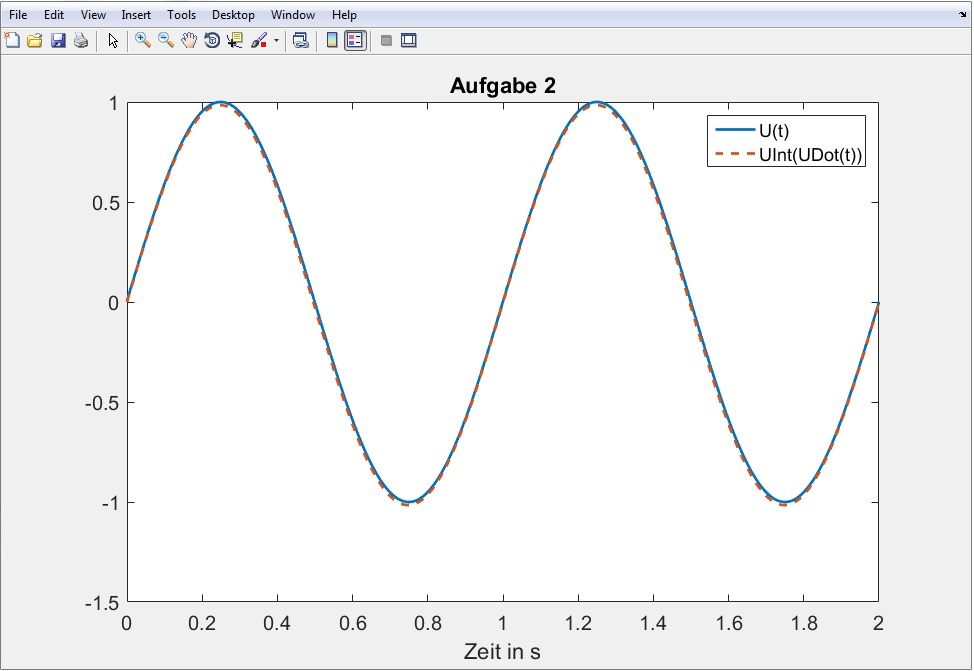
\includegraphics[width=\textwidth]{plot2.png}
\caption{Plot}
\label{fig4}
\end{figure}

Dazu wurden folgende Befehle verwendet:

\lstinputlisting[language=Matlab]{Aufgabe1C2.m}

\newpage



\end{document}
